\documentclass{article}

\usepackage{amsmath, amsthm}
\usepackage{setspace}
\usepackage{microtype, parskip}
\usepackage[comma,sort&compress]{natbib}
\usepackage{lineno}
\usepackage{docmute}
\usepackage{caption, subcaption, multirow, morefloats, rotating}
\usepackage{wrapfig}

\frenchspacing

\doublespacing

\raggedright

\begin{document}
\linenumbers
\modulolinenumbers[2]

%\maketitle

\begin{titlepage}
  \begin{large}
    \textbf{Title:} How macroecology affects macroevolution: the interplay between extinction intensity and trait-dependent extinction in brachiopods.
  \end{large}

  \textbf{Running title:} Trait-dependent extinction in brachiopods

  \textbf{Author:} Peter D Smits, psmits@uchicago.edu, Committee on Evolutionary Biology, University of Chicago, IL, USA.

  \textbf{Keywords:} species selection, paleobiology, Bayesian

  \textbf{Word count:} \(\approx\) 7000
  
  \textbf{Table count:} 1
 
  \textbf{Figure count:} 7

  \textbf{Data archival location:} Zenodo DOI 10.5281/zenodo.46928.

\end{titlepage}

\begin{abstract}
  As extinction intensity increases, how do the effects of traits on taxonomic survival change? Does the extinction rate associated with certain traits increase while that of others decreases? Using a hierarchical Bayesian approach, I develop a model of how the effects of biological traits on extinction risk can vary with respect to extinction intensity, origination cohort (i.e. time of origination), and in relation to each other. The emergent traits traits I analyze in relation to their patterns of Paleozoic brachiopod genus durations are geographic range, affinity for epicontinental seas versus open ocean environments, and body size. Additionally, I estimate the effects of environmental generalization versus specialization on taxonomic survival by allowing environmental preference to have a nonlinear effect on duration. My analytical framework eschews the traditional distinction between background and mass extinction, and instead considers extinction intensity as a continuum. I find that the cohort-specific effects of geographic range and environmental preference are negatively correlated with baseline extinction intensity. Additionally, I find support for greater survival of environmental generalists versus specialists in all origination cohorts. These results support the conclusion that for Paleozoic brachiopods, as extinction intensity increases overall extinction selectivity increases.
\end{abstract}


\section{Introduction}

Extinction is one half of the diversification process \citep{Raup1994,Stanley1979,Stanley1975}, second only to speciation or origination; it can also be the ultimate manifestation of selection as a taxon with a beneficial trait should persist for longer on average than a taxon without that beneficial trait \citep{Rabosky2010b,Jablonski2008a,Raup1994,Stanley1975}. 

While estimation of both trait-dependent speciation and extinction rates from phylogenies of extant taxa has grown dramatically \citep{Maddison2007,Fitzjohn2010,Goldberg2011a,Goldberg2005,Rabosky2013,Stadler2013b,Stadler2011a,Stadler2013a}, there are two major ways to estimate trait-dependent extinction: analysis of phylogenies, and analysis of the fossil record. These two directions, phylogenetic comparative and paleobiological, are complementary and intertwined in the field of macroevolution \citep{Rabosky2010b,Jablonski2008a,Hunt2014a}. In the case of extinction, analysis of the fossil record has the distinct advantage over phylogenies of only extant taxa because extinction is observable; this means that extinction rate is possible to estimate \citep{Rabosky2010a,Quental2009,Liow2010a}. The approach used here is thus complementary to the analysis of trait-dependent extinction based on a phylogeny.

\citet{Jablonski1986} observed that for bivalves at the end Cretaceous mass extinction event, the effects of some biological traits on taxonomic survival decreased. However, this pattern was not the case for the effect of geographic range on survival \citep{Jablonski1986,Payne2007}. There are multiple possible macroevolutionary mechanisms which may underlie this pattern: the effect of geographic range on survival remains constant and those of other biological traits decrease, the effect of geographic range on survival increases and those of other biological traits stay constant, or the effects of all traits decrease potentially by different degrees.

While \citet{Jablonski1986} phrased his conclusions in terms of background versus mass extinction, these states are not distinguishable in terms of extinction rate alone; my analysis treats the time period analyzed as part of the same continuum \citep{Wang2003,Payne2007,Simpson2009}. Additionally, in order to test the proposed macroevolutionary mechanism behind the \citet{Jablonski1986} scenario; not only do the taxon trait effects needs to be modeled, but the correlation between trait effects need to be modeled as well. 

Here I model brachiopod taxon durations because trait based differences in extinction risk should manifest as differences in taxon durations. Brachiopods are an ideal group for this study as they are are well known for having an exceptionally complete fossil record \citep{Foote1996e,Foote2000a}. I focus on the brachiopod record from the post-Cambrian Paleozoic, from the start of the Ordovician (approximately 485 My) through the end Permian (approximately 252 My) as this represents the time of greatest global brachiopod diversity \citep{Alroy2010} meaning a large sample size for this analysis.

The analysis of taxon durations, or time from origination to extinction, falls under the purview of survival analysis, a field of applied statistics commonly used in health care and engineering \citep{Klein2003} but has a long history in paleontology \citep{Simpson1944,Simpson1953,VanValen1973,VanValen1979,Crampton2016}. I adopt a hierarchical modeling approach \citep{Gelman2007,Gelman2013d}, which represents both a conceptual and statistical unification of the paleontological dynamic and cohort survival analytic approaches \citep{VanValen1973,VanValen1979,Raup1978,Raup1975,Foote1988,Baumiller1993,Simpson2006,Crampton2016,Ezard2012b}. 

\subsection{Factors affecting brachiopod survival}

Conceptually, taxon survival can be considered an aspect of ``taxon fitness'' \citep{Cooper1984,Palmer2012}. Traits associated with taxon survival are thus examples of species (or higher-level) selection, as differences in survival are analogous to differences in fitness. The traits analyzed here are all examples of emergent and aggregate traits \citep{Jablonski2008a,Rabosky2010b}; specifically I analyze genus-level traits. Emergent traits are those which are not measurable at a lower level (e.g. species versus individual organism) such as geographic range, or even fossil sampling rate. Aggregate traits, like body size or environmental preference, are the average of a shared trait across all members of a lower level.

Geographic range is widely considered the most important biological trait for estimating differences in extinction risk at nearly all times, with large geographic range associated with low extinction risk \citep{Jablonski1986,Jablonski1987,Jablonski2003,Payne2007,Jablonski2008a,Harnik2013,Finnegan2012a}. This stands to reason even if extinction is completely at random; a taxon with an unrestricted range is less likely to go extinct at random than a taxon with a restricted range.

Epicontinental seas are a shallow-marine environment where the ocean has spread over the continental interior or craton with a depth typically less than 100m. In contrast, open-ocean coastline environments have much greater variance in depth, do not cover the continental craton, and can persist during periods of low sea level \citep{Miller2009a}. Because of this, a simple hypothesis that taxa which favor epicontinental seas would be at great risk during periods of low sea levels, such as during glacial periods, when epicontinental seas are drained. During the Paleozoic (approximately 541--252 My), epicontinental seas were widely spread globally but declined over the Mesozoic (approximately 252--66 My) and have nearly disappeared during the Cenozoic (approximately 66--0 My) as open-ocean coastlines became the dominant shallow-marine setting \citep{Sheehan2001b,Peters2008,Miller2009a,Johnson1974}. Taxa in epicontinental environments could also have a greater extinction susceptibility than taxa in open-ocean environments due to anoxic events due to enhanced water stratification or poor water circulation \citep{Peters2007}.

\citet{Miller2009a} demonstrated that during several mass extinctions taxa associated with open-ocean environments tend to have a greater extinction risk than those taxa associated with epicontinental seas. During periods of background extinction, however, they found no consistent difference between taxa favoring either environment. \citet{Miller2009a} hypothesize that open-ocean taxa may have a greater extinction rate because these environments would be more strongly affected by waterborne hazards such as fallout from impacts or volcanic events which would propagate more quickly than in epicontinental environments with sluggish circulation. These two environment types represent the primary identifiable environmental dichotomy observed in ancient marine systems \citep{Miller2009a,Sheehan2001b}. Given these findings, I would hypothesize that as extinction risk increases, the extinction risk associated with open-ocean environments should generally increase. 

Because environmental preference is defined here as the continuum between occurring exclusively in open-ocean environments versus epicontinental environments, intermediate values are considered ``generalists'' in the sense that they favor neither end member. A long-standing hypothesis is that generalists or unspecialized taxa will have greater survival than specialists \citep{Simpson1944,Liow2004a,Liow2007b,Nurnberg2013a,Nurnberg2015,Baumiller1993,Smits2015}. Because of this, the effect of environmental preference was modeled as a quadratic function where a concave down relationship between preference and expected duration indicates that generalists are favored over specialists end-members.

Body size, measured as shell length, is also considered as a trait that may potentially influence extinction risk \citep{Payne2014,Harnik2011}. Body size is a proxy for metabolic activity and other correlated life history traits \citep{Payne2014}. \citet{Harnik2014} analyzed the effect of body size selectivity in Devonian brachiopods in both a phylogenetic and non-phylogenetic context; finding that body size was not found to be associated with differences in taxonomic duration. It has also been found that, at least in the case of some bivalve subclades, body size can be as important a factor as geographic range size in determining extinction risk \citep{Harnik2011}. Given these results, I expect that if body size has any effect on brachiopod taxonomic survival it is very small.

It is well known that, given the incompleteness of the fossil record, the observed duration of a taxon is an underestimate of that taxon's true duration \citep{Solow1997,Wagner2013a,Wang2004,Liow2010b,Alroy2014a,Foote1996e}. Because of this, the concern is that a taxon's observed duration may reflect its relative chance of being sampled and not any of the effects of the covariates of interest. In this case, for sampling to be a confounding factor there must be consistent relationship between the quality of sampling of a taxon and its apparent duration (e.g. greater sampling, longer duration). If there is no relationship between sampling and duration then interpretation can be made clearly; while observed durations are obviously truncated true durations, a lack of a relationship would indicate that the amount and form of this truncation is not a major determinant of the taxon's apparent duration. By including sampling as a covariate in the model, this effect can be quantified and can be taken into account when interpreting the estimates of the effects of the other covariates.



\section{Materials and Methods}

\subsection{Fossil occurrence information}

% foote gave me a hand with the taxonomic occurrences
%   biggest limiting factor is the Payne 2014 body size dataset
The brachiopod dataset analyzed here was sourced from the Paleobiology Database (http://www.paleodb.org) which was then filtered based on taxonomic (Rhychonelliformea: Rhynchonellata, Chileata, Obolellida, Kutorginida, Strophomenida, Spiriferida), temporal (post-Cambrian Paleozoic), stratigraphic, and other occurrence information used in this analysis. Analyzed occurrences were restricted to those with paleolatitude and paleolongitude coordinates, assignment to either epicontinental or open-ocean environment, and belonging to a genus present in the body size dataset \citep{Payne2014}. Epicontinental versus open-ocean assignments for each fossil occurrence are partially based on those from \citet{Miller2009a}, with additional occurrences assigned similarly (Miller and Foote, personal communication). These filtering criteria are very similar to those from \citet{Foote2013} with an additional constraint of being present in the body size data set from \citet{Payne2014}. In total, there 1130 were genera included in the dataset.

% justification of using genus level versus specific
Fossil occurrences were analyzed at the genus level which is common for paleobiological, macroevolutionary and macroecological studies of marine invertebrates \citep{Alroy2010,Foote2013,Harnik2013,Kiessling2007a,Miller2009a,Nurnberg2013a,Nurnberg2015,Payne2007,Simpson2009,Vilhena2013}. While species diversity dynamics are frequently of much greater interest than those of higher taxa (though see \citealt{Foote2014b,Hoehn2015}), the nature of the fossil record makes accurate, precise, and consistent taxonomic assignments at the species level difficult for all occurrences. As such, the choice to analyze genera as opposed to species was in order to assure a minimum level of confidence and accuracy in the data analyzed here.

Genus duration was calculated as the number of geologic stages from first appearance to last appearance, inclusive. Durations were based on geologic stages as opposed to millions of years because of the inherently discrete nature of the fossil record; dates are not assigned to individual fossils themselves but instead fossils are assigned to a geological interval which represents some temporal range. In this analysis, stages are effectively irreducible temporal intervals in which taxa may occur. Genera with a last occurrence in or after Changhsingian stage (e.g. the final stage of the study interval) were right censored at the Changhsingian; genera with a duration of only one stage were left censored \citep{Klein2003}. How the likelihood of censored observations is calculated is detailed in section \ref{sec:model}.

The covariates of duration included in this analysis are geographic range size (\(r\)), environmental preference (\(v, v^{2}\)), body size (\(m\)), and sampling (\(s\)).

Geographic range was calculated as relative occupancy corrected for incomplete sampling. First, the paleolatitude-paleolongitude coordinates for all occurrences were projected onto an equal-area cylindrical map projection. Each occurrence was then assigned to one of the cells from a 70 \(\times\) 34 regular raster grid placed on the map. Each grid cell represents approximately 250,000 km\(^{2}\). The map projection and regular lattice were made using shape files from http://www.naturalearthdata.com/ and the \texttt{raster} package for R \citep{raster}. For each stage, the total number of occupied grid cells was calculated. Then, for each temporal bin, the relative occurrence probability of the observed taxa was calculated using the \uppercase{jade} method developed by \citet{Chao2015a}. This method accounts for the fact that taxa with an occupancy of 0 cannot be observed which means that occupancy follows a truncated Binomial distribution. This correction is critical when comparing occupancies from different times with different geographic sampling. Finally, for each genus, the mean relative occurrence probability was calculated as the average of that genus' occurrence probabilities for all stages it was sampled to yield relative occupancy, my proxy for geographic range.

Environmental preference was defined as probability of observing the ratio of epicontinental occurrences to total occurrences (\(\theta_{i} = e_{i} / E_{i}\)) or greater given the background occurrence probability \(\theta^{\prime}_{i}\) as estimated from all other taxa occurring at the same time (\(e^{\prime}_{i} / E^{\prime}_{i}\)). This measure of environmental preference is expressed.
\begin{equation}
  \begin{aligned}
    p\left(\theta^{\prime}_{i} \middle| e^{\prime}_{i}, E^{\prime}_{i} \right) &\propto \mathrm{Beta}(e^{\prime}_{i}, E^{\prime}_{i} - e^{\prime}_{i}) \mathrm{Beta}(1, 1) \\
    &= \mathrm{Beta}(e^{\prime}_{i} + 1, E^{\prime}_{i} - e^{\prime}_{i} + 1),
  \end{aligned}
  \label{eq:envpref}
\end{equation}
where \(v\) is the percent of the distribution defined in equation \ref{eq:envpref} less than or equal to \(\theta_{i}\). The Beta distribution is used here because it is a continuous distribution bounded at 0 and 1, which is idea for modeling percentages.

Body size, measured as shell length, was sourced directly from \citet{Payne2014}. These measurements were made from brachiopod taxa figured in the \textit{Treatise on Invertebrate Paleontology} \citep{Brunton2007}.

The sampling probability for individual taxa was calculated using the standard gap statistic \citep{Foote1996e,Foote2000}. The gap statistic is calculated as the number of stages in which the taxon was sampled minus two divided by the duration of the taxon minus two. Subtracting two from both the numerator and denominator is because the first and last appearance stages are by definition sampled. Because taxa that were right censored only include a first appearance, one was subtracted from the numerator and denominator instead of two.

The minimum duration for which a gap statistic can be calculated is three stages, so I chose the impute the gap statistic for all observations with a duration less than 3. Imputation is the ``filling in'' of missing observations based on the observed values \citep{Rubin1996,Gelman2007}. This is fairly straight forward in a Bayesian framework because both covariates and parameters are considered random variables, meaning that the missing values of sampling can be modeled as coming from some probability distribution. The model for imputing sampling probability is described in section \ref{sec:impute}.

Prior to analysis, geographic range was logit transformed and body size was natural-log transformed; both of these transformations make these variables defined for the entire real line. Sampling probability was transformed as \((s (n - 1) + 0.5) / n\) where \(n\) is the sample size as recommended by \citet{Smithson2006}; this serves to slightly shrink the range of the data so that there are no values of 0 or 1. All covariates except for sampling were standardized by subtracting the mean from all values and dividing by twice its standard deviation, which follows \citet{Gelman2007}. This standardization means that the associated regression coefficients are comparable as the expected change per 1-unit change in the rescaled covariates. Finally, \(D\) is defined as the total number of covariates, excluding sampling, plus one for the intercept term.



\subsection{Details of model}
\label{sec:model}

% hierarchical modeling is simply modeling the hyperparameters of a prior distribution
%   Gelman2013d
% observed outcomes are conditioned on certain parameters which are themselves modeled
Hierarchical modelling is a statistical approach which explicitly takes into account the structure of the observed data in order to model both the within and between group variance \citep{Gelman2013d,Gelman2007}. The units of study (e.g. genera) each belong to a single group (e.g. origination cohort). Each group is considered a draw from a shared probability distribution (e.g. prior) of all cohorts, observed and unobserved. The group-level parameters, or the hyperparameters of this shared prior, are themselves given (hyper)prior distributions and are also estimated like the other parameters of interest (e.g. covariate effects) \citep{Gelman2013d}. The subsequent estimates are partially pooled together, where parameters from groups with large samples or effects remain large while those of groups with small samples or effects are pulled towards the overall group mean. All covariate effects (regression coefficients), as well as the intercept term (baseline extinction risk), were allowed to vary by group (origination cohort). The covariance between covariate effects was also modeled. 

Genus durations were assumed to follow a Weibull distribution which allows for age-dependent extinction \citep{Klein2003}: \(y \sim \mathrm{Weibull}(\alpha, \sigma)\). The Weibull distribution has two parameters: scale \(\sigma\), and shape \(\alpha\). When \(\alpha = 1\), \(\sigma\) is equal to the expected duration of any taxon. \(\alpha\) is a measure of the effect of age on extinction risk where values greater than 1 indicate that extinction risk increases with age, and values less than 1 indicate that extinction risk decreases with age. Note that the Weibull distribution is equivalent to the exponential distribution when \(\alpha = 1\). 

In the case of the right- and left-censored observations mentioned above, the probability of those observations has a different calculation \citep{Klein2003}. For right-censored observations, the likelihood is calculated \(p(y | \theta) = 1 - F(y) = S(y)\) where \(F(y)\) is the cumulative distribution function. In contrast, the likelihood of a left-censored observation is calculated \(p(y | \theta) = F(y)\).

The scale parameter \(\sigma\) was modeled as a regression following \citet{Kleinbaum2005} with both varying intercept and varying slopes and the effect of sampling; this is expressed
\begin{equation}
  \sigma_{i} = \exp\left(\frac{-\mathbf{X}_{i} B_{j[i]} + \delta s_{i}}{\alpha}\right)
  \label{eq:sigma}
\end{equation}
where \(i\) indexes across all observations where \(i = 1, \dots, n\) where \(n\) is the total number of observations, \(j[i]\) is the cohort membership of the \(i\)th observation where \(j = 1, \dots, J\) where \(J\) is the total number of cohorts, \(X\) is a \(N \times D\) matrix of covariates along with a column of 1's for the intercept term, \(B\) is a \(J \times D\) matrix of cohort-specific regression coefficients, and \(\delta\) is the regression coefficient for the effect of sampling \(s\). \(\delta\) does not vary by cohort.

Each of the rows of matrix \(B\) are modeled as realizations from a multivariate normal distribution with length \(D\) location vector \(\mu\) and \(J \times J\) covariance matrix \(\Sigma\): \(B_{j} \sim \mathrm{MVN}(\mu, \Sigma)\). The covariance matrix was then decomposed into a length \(J\) vector of scales \(\tau\) and a \(J \times J\) correlation matrix \(\Omega\), defined \(\Sigma = \mathrm{diag}(\tau) \Omega \mathrm{diag}(\tau)\) where ``diag'' indicates a diagonal matrix.

The elements of \(\mu\) were given independent normally distributed priors. The effects of geographic range size  and the breadth of environmental preference were given informative priors reflecting the previous findings while the others were given weakly informative favoring no effect. The correlation matrix \(\Omega\) was given an LKJ distributed prior \citep{Lewandowski2009} that slightly favors an identity matrix as recommended by \citet{stan-manual:2014}. These priors are defined
\begin{equation}
  \begin{aligned}
    \mu^{0} &\sim \mathcal{N}(0, 5) \\
    \mu^{r} &\sim \mathcal{N}(-1, 1) \\
    \mu^{v} &\sim \mathcal{N}(0, 1) \\
    \mu^{v^{2}} &\sim \mathcal{N}(1, 1) \\
    \mu^{m} &\sim \mathcal{N}(0, 1) \\
    \tau &\sim \mathrm{C^{+}}(1) \\
    \Omega &\sim \text{LKJ}(2).
  \end{aligned}
  \label{eq:sigma_prior}
\end{equation}

The log of the shape parameter \(\alpha\) was given a weakly informative prior \(\log(\alpha) \sim \mathcal{N}(0, 1)\) centered at \(\alpha = 1\), which corresponds to the Law of Constant Extinction \citep{VanValen1973}.

\subsection{Imputation of sampling probability}
\label{sec:impute}
% Unknown values were estimated from the results of that beta regression.
The vector sampling \(s\) has two parts: the observed part \(s^{o}\), and the unobserved part \(s^{u}\). Of the 1130 total observations, 539 have a duration of 3 or more and have an observed gap statistic. The gap statistic for the remaining 591 observations was imputed. As stated above, the unobserved part is the imputed, or filled in, based on the observed part \(s^{o}\). Because sampling varies between 0 and 1, I chose to model it as a Beta regression with matrix \(W\) being a \(N \times (D - 1)\) matrix of covariates (i.e. geographic range size, environmental preference, body size) as predictors of sampling; this assumes that the sampling value for all taxa come from the same distribution. Importantly, I make no assumptions of causal structure. 

Predicting sampling probability using the other covariate that are then included in the model of duration is acceptable and appropriate in the case of imputation where the sample goal is accurate prediction \citep{Rubin1996,Gelman2007}. Not including these covariates can lead to biased estimates of the imputed variable; if the covariates themselves are related, not including them will bias this correlation towards zero which then leads to improper imputation and inference \citep{Rubin1996}.

The Beta regression is defined
\begin{equation}
  s^{o} \sim \mathrm{Beta}(\phi = \text{logit}^{-1}(X^{o} \gamma), \lambda),
  \label{eq:impute}
\end{equation}
where \(\gamma\) is a length \(D\) vector of regression coefficients, and \(X\) defined as above. The Beta distribution used in the regression is reparameterized in terms of a mean parameter
\begin{equation}
  \phi = \frac{\alpha}{\alpha + \beta}
\end{equation}
and total count parameter
\begin{equation}
  \lambda = \alpha + \beta
\end{equation}
where \(\alpha\) and \(\beta\) are the characteristic parameters of the Beta distribution \citep{Gelman2013d}.

The next step is to then estimate \(s^{u} | s^{o}, X^{o}, X^{u}, \gamma\), the posterior distribution of which are folded back into \(s\) and used as a covariate of duration (Eq. \ref{eq:sigma}). All the elements of \(\gamma\), and both \(\delta\) (Eq. \ref{eq:sigma}) and \(\lambda\) (Eq. \ref{eq:impute}) were given weakly informative priors where
\begin{equation}
  \begin{aligned}
    \gamma &\sim \mathcal{N}(0, 1) \\
    \delta &\sim \mathcal{N}(0, 1) \\
    \lambda &\sim \mathrm{Pareto}(0.1, 1.5). \\
  \end{aligned}
\end{equation}


%The above model is for all taxa and does not include sampling as a covariate. In order to determine if sampling is acting as a confounding factor in this analysis, an additional model was developed because sampling was only estimated for taxa with a duration of three or more which creates a left-truncated distribution of durations \citep{Klein2003}. The sampling statement and log-probability for a left-truncated Weibull distribution, truncated at time \(Y\) (e.g. three), is
%\begin{equation}
%  \begin{aligned}
%    p(y | \theta) &= \frac{\mathrm{Weibull}(y, \alpha, \sigma)}{1 - \mathrm{Weibull}_{cdf}(Y, \alpha, \sigma)} \\
%    &= \frac{\mathrm{Weibull}(y, \alpha, \sigma)}{\mathrm{Weibull}_{ccdf}(Y, \alpha, \sigma)} \\
%    \log(p(y | \theta)) &= \log(\mathrm{Weibull}(y, \alpha, \sigma)) - \log(\mathrm{Weibull}_{ccdf}(Y, \alpha, \sigma)).
%  \end{aligned}
%  \label{eq:trunc}
%\end{equation}
%Note that cdf stands for cumulative distribution function and ccdf is the complementary cumulative distribution function.
%
%The definition of \(\sigma\) (Eq. \ref{eq:sigma}) is then updated so that \(X\), the matrix of covariates, and \(B\), the matrix of regression coefficients, now include an additional column for the sampling estimates and the cohort-specific effects of sampling. This addition then modifies the dimensions of \(\mu\) and \(\Sigma\); the new group-level effect of \(\mu^{s}\) is given a weakly informative prior: \(\mu^{s} \sim \mathcal{N}(0, 1)\).
%
%For this left-truncated model, I've excluded one observation that is right-censored with a duration equal to the truncation time; the second line of equation \ref{eq:trunc} becomes \(p(y | \theta) = \mathrm{Weibull}_{ccdf}(y, \alpha, \sigma) / \mathrm{Weibull}_{ccdf}(Y, \alpha, \sigma)\) which yields a log-probability of 0.


\subsection{Posterior inference and posterior predictive checks}
The joint posterior was approximated using a Markov-chain Monte Carlo routine that is a variant of Hamiltonian Monte Carlo called the No-U-Turn Sampler \citep{Hoffman2014} as implemented in the probabilistic programming language Stan \citep{2014stan}. The posterior distribution was approximated from four parallel chains run for 10,000 steps each, split half warm-up and half sampling and thinned to every 10th sample for a total of 4000 posterior samples. Chain convergence was assessed via the scale reduction factor \(\hat{R}\) where values close to 1 (\(\hat{R} < 1.1\)) indicate approximate convergence. Convergence means that the chains are approximately stationary and the samples are well mixed \citep{Gelman2013d}.

% edit, relab, and impute can all be compared using WAIC/PSIS-LOO
%   highgrade cannot
%The fit of the above model (the ``full'' model) was compared to the fits of three other sub-models: constant \(\alpha\) across cohorts, no sampling as a covariate, or both constant \(\alpha\) and no sampling covariate. These models were compared for predicted out-of-sample predictive accuracy using both the widely-applicable information criterion (WAIC) and leave-one-out cross-validation estimated via Pareto-smoothed importance sampling (PSIS-LOO) \citep{Vehtari2015}. Both of these are estimates of the out-of-sample predictive accuracy or the expected quality of fit of the model to new data. 
%
%WAIC is a more fully Bayesian alternative to AIC or DIC \citep{Watanabe2010a,Gelman2013d}; comparisons of WAIC values are useful for better understanding the effect of model complexity on out-of-sample predictive accuracy. Note that BIC is not an estimate of out-of-sample predictive accuracy \citep{Gelman2013d}. The calculation of WAIC used here corresponds to the ``WAIC 2'' formulation recommended by \citet{Gelman2013d}. Lower values of WAIC indicate greater expected out-of-sample predictive accuracy than higher values.
%
%PSIS-LOO is similar to WAIC in that it is an approxmiation of out-of-sample predictive accuracy except its calculation is completely different \citep{Vehtari2015,Vehtari2015a}. Models comparison is done using a leave-one-out crossvalidation information criterion (LOOIC), which is simply the PSIS-LOO estimate multiplied by -2 so that it is on the deviance scale. As with WAIC, models with lower values of LOOIC are expected to have a greater out-of-sample predictive accuracy than models with greater values.
%
%Calcuations of WAIC and PSIS-LOO for a model fit using Stan were done using the R package ``loo'' \citep{loo}. See \citet{Vehtari2015a} for detailed explinations of the calucations for both WAIC and PSIS-LOO.

Model adequacy was evaluated using a couple of posterior predictive checks. Posterior predictive checks are a means for understanding model fit or adequacy where the basic idea is that replicated data sets simulated from the fitted model should be similar to the original data and systematic differences between the simulations and observations indicate weaknesses of the model fit \citep{Gelman2013d}. For both approaches used here, each posterior predictive datasets were generated from a unique draw from the posterior distribution of each parameter. The two posterior predictive checks used in this analysis are a comparison of a non-parametric estimate of the survival function \(S(t)\) from the empirical dataset to the non-parametric estimates of \(S(t)\) from the 100 posterior predictive datasets, and comparison of the observed genus durations to the average posterior predictive estimate of \(\log(\sigma)\) (Eq. \ref{eq:sigma}). The former is to see if simulated data has a similar survival pattern to the observed, while the latter is to see if the model systematically over- or under- estimates taxon survival.

% everything is on zenodo if you want to reproduce this entire analysis
% All code necessary to reproduce this analysis are available through an archived Zenodo repository DOI URL.



\section{Results}

Comparison of the posterior predictive estimates of \(S(t)\) to the empirical estimate reveal few obvious biases except for the case of values from the far right tail of observed durations (Fig. \ref{fig:surv}). This result is reinforced by the additional posterior predictive comparison where most estimates are not systematically biased except for a consistent under-estimate of \(\log(\sigma)\) for older taxa (Fig. \ref{fig:shot}). The results of both posterior predictive checks indicate that, for the majority of observations, model fit is generally not biased.

The cohort-level estimate of the effect of geographic range size indicates that as a taxon's geographic range increases, that taxon's duration is expected to increase (Table \ref{tab:param}). Given the estimates of \(\mu^{r}\) and \(\tau^{r}\), there is a less than 3.7\% (\(\pm 0.04\%\) SD) probability that this relationships would be reversed (\(\mathrm{Pr}\mathcal{N}(\mu^{r}, \tau^{r}) > 0)\)). The between-cohort variance \(\tau^{r}\) is the lowest of all the regression coefficients (Table \ref{tab:param}).

Body size is estimated to have no effect on taxon duration, with the estimate being nearly 0 (Table \ref{tab:param}). The variance between the cohort-specific estimates of the effect of body size \(\tau^{m}\) is estimated to be greater than the variance of between-cohort estimates of the effect of geographic range size \(\tau^{r}\). 

The group-level estimate of the effect of environmental preference is estimated from both \(\mu^{v}\) and \(\mu^{v^{2}}\). 

The estimate of \(\mu^{v}\) indicates that epicontinental favoring taxa are expected to have a greater duration than open-ocean favoring taxa (Table \ref{tab:param}). Additionally, given the estimate of between-cohort variance \(\tau^{v}\), there is approximately 18\% (\(\pm 7\%\) SD) probability that, for any given cohort, taxa favoring open-ocean environments would have a greater expected duration than taxa favoring epicontinental environments (\(\mathrm{Pr}(\mathcal{N}(\mu^{v}, \tau^{v}) > 0)\)). 

The estimate of \(\mu^{v^{2}}\) indicates that the overall relationship between environmental preference and \(\log(\sigma)\) is concave down (Fig. \ref{fig:env_mean}), with only a 2.7\% (\(\pm 3\%\) SD) probability that any given cohort is convex up (\(\mathrm{Pr}(\mathcal{N}(\mu^{v^{2}}, \tau^{v^{2}}) < 0\)).

The cohort-specific estimates of all the regression coefficients demonstrate a lot of between cohort variance, with no obvious trends. As indicated in Table \ref{tab:param} and detectable visually (Fig. \ref{fig:cohort_series}), the between-cohort estimates for \(\beta^{0}\), \(\beta^{r}\), and \(\beta^{m}\) all have much lower variance than the between-cohort estimates of both \(\beta^{v}\) and \(\beta^{v^{2}}\).

While most cohort-specific estimates are very similar to the overall cohort-level estimate, there are a few notable excursions away from the overall mean (Fig. \ref{fig:cohort_series}). There are simultaneous excursions in both \(\beta^{0}\) and \(\beta^{v}\) for cohorts originating in the Givetian (387-382 My) and Frasnian (382-372 My) stages; both of which directly precede the late Devonian mass extinction event at the Frasnian/Famennian boundary. These cohorts are marked by both a high extinction intensity and an increase in expected duration for taxa favoring epicontinental environments over open-ocean ones; this is consistent with the results of \citet{Miller2009a}.

Cohorts originating from the Silurian through the Early Devonian have a slightly lower extinction intensity than the overall mean; these cohorts are those originating in the Llandovery (443-443 My) through the Emsian (407-393 My). This is also a time period is also when there is the lowest overall probability that epicontinental favoring taxa are expected to have greater duration than open-ocean favoring taxa. Both the Silurian and Devonian periods are notable for having been periods with a mostly ``hothouse'' climate, with no polar icecaps and a high sea-level \citep{Edwards1985,Joachimski2009,Munnecke2010}.
% Probability inflection point > 0 for cohorts 6 (Kantian) through 15 (Eifelian):
%   0.99, 0.99, 0.632, 0.377, 0.685, 0.754, 0.52, 0.851, 0.581, 0.995

% cohort-specific environmental effect
%   description of the variation in estimates
%   mass extinction boundaries
The cohort-specific relationships between environmental preference and \(\log(\sigma)\) were calculated from the estimates of \(\beta^{0}\), \(\beta^{v}\), and \(\beta^{v^{2}}\) (Fig. \ref{fig:env_cohort}) and reflect how these three parameters act in concert and not just individually (Fig. \ref{fig:cohort_series}). Beyond results already discussed above in the context of the parameters individually, it is notable that the cohort originating in the Kungurian (279-272 My) is least like the overall expected relationship and has the most sharply curved appearance due to a high estimate \(\beta^{v^{2}}\) (Fig. \ref{fig:cohort_series}). This cohort has the biggest difference in extinction risk between environmental generalists and specialists. The cohorts originating during the Emsian (407-393 My) and Frasnian (382 - 372 My) are tied for second in sharpness of curvature. The least sharply curved cohorts include those originating during Tremadocian (484-477 My), Hirnantian (445-443 My), Llandovery (443-433 My), and Ludlow (427-423 My). Except for the Tremadocian cohort, most of these cohorts originate during the Silurian through the Early Devonian range identified earlier as having lower expected extinction intensity than what is expected from the group-level estimate.

The correlations of the cohort-specific estimates of the regression coefficients are estimated as the off-diagonal elements of the correlation matrix \(\Omega\). Only two of the elements of \(\Omega\) are distinguishable from 0: the correlation of \(\beta^{0}\) (extinction intensity) with both \(\beta^{r}\) and \(\beta^{v}\) (Fig. \ref{fig:cor_posterior}). 

There is an approximate 90\% probability that the cohort-specific estimates of baseline extinction intensity \(\beta^{0}\) and the effect of geographic range \(\beta^{r}\) are negatively correlated; this means that for cohorts experiencing a lower extinction intensity (\(\beta^{0}\) decreases), the magnitude of the effect of geographic range is expected to decrease as well, and \textit{vice versa}; this is in contrast to the observation made by \citet{Jablonski1986} with regards to late Cretaceous bivalves.

Similarly, there is an approximate 97.4\% probability that the cohort-specific estimates of \(\beta^{0}\) and \(\beta^{v}\) are negatively correlated; this means that as extinction intensity increases it is expected that epicontinental taxa become more favored over open-ocean environments (i.e. as \(\beta^{0}\) increases, \(\beta^{v}\) decreases). 

There is only an approximate 30\% probability that \(\beta^{r}\) and \(\beta^{v}\) are positively correlated. This lack of cross-correlation may be due in part to the much higher between-cohort variance of the effect of environmental preference \(\tau^{v}\) than the very small between-cohort variance in the effect of geographic range \(\tau^{r}\) (Table \ref{tab:param}); the effect of geographic range might simply not vary enough relative to the much noisier environmental preference.

Comparison of observed values of sampling, as measured by the gap statistic, to random draws from the posterior estimates of the imputed sampling values indicate that they are very similar (Fig. \ref{fig:impute_results}. This result is very encouraging as this is the ultimate goal of multiple imputation: to fill in missing data with values similar to the observed while taking into account the randomness of that variable \citep{Rubin1996,Gelman2007}. The estimates of \(\delta\) are based on the set of observed values and the entire posterior of imputed values.

Sampling was found to have a negative effect (positive \(\delta\)) on duration: greater sampling, shorter duration (Table \ref{tab:param}). While potentially counter intuitive, this result is most likely due to some long lived taxa only be sampled in the stages of the first and last appearance. Also, longer lived taxa have more opportunities to not be sampled than shorter lived taxa. These two factors will lead to this result. 

While the effect of sampling appears large compared to the other regression coefficients, this is only because sampling was not standardized like the other covariates. To make the coefficients comparable, \(\delta\) is multiplied by twice the posterior mean of the standard deviation of sampling probability; the transformed value of \(\delta\) is then 0.642 (\(\pm 0.1\) SD). This effect is relatively small compared to the other covariate effects (Table \ref{tab:param}). There is then a 98.6\% probability that the effect of geographic range \(\mu^{r}\) has a greater magnitude than \(\delta\). Similarly, \(\mu^{v}\) has a 71.8\% probability of having a greater magnitude of effect than \(\delta\). Finally, \(\mu^{v^{2}}\) has a 100\% probability of having a greater magnitude of effect than \(\delta\).

The Weibull shape parameter \(\alpha\) was found to be approximately 1.36 (\(\pm 0.05\) SD) with a 100\% probability of being greater than 1. This result is not consistent with the Law of Constant Extinction \citep{VanValen1973} and is instead consistent with accelerating extinction risk with taxon age. This may indicate that older taxa are out-competed by younger taxa, a result consistent with some empirical results \citep{Wagner2014b,Quental2013,Smits2015} and (ironically) with a recently proposed Red Queen-like model of evolution \citep{Rosindell2015a}. This results, however, is not consistent with other empirical results \citep{Finnegan2008,Crampton2016} and could potentially be caused by the minimum resolution of the fossil record \citep{Sepkoski1975}. It is thus unclear if a strong biological inference can be made from this result, which means that further work is necessary on the effect of taxon age on extinction risk.


\section{Discussion}

The generating observation behind this study was that for bivalves at the end Cretaceous mass extinction event, the only biological trait that was found the affect extinction risk was geographic range while traits that had previously been beneficial had no effect \citep{Jablonski1986}. This observation raises two linked questions: how does the effect of geographic range change with changing extinction intensity, and how does the effect of other biological traits change with changing extinction intensity?

I find that as intensity increases (\(\beta^{0}\) decreases), the magnitude of the effect of geographic range increases. I also find that as intensity increases, the effect of favoring epicontinental environments of open-ocean environments is expected to be increase; this is consistent with the results of \citet{Miller2009a}. There is no evidence for a correlation between the effect of geographic range and environmental preference. Additionally, the between-cohort variance in effect of geographic range is much less then the between-cohort variance of the effect of environmental preference which may underlie the lack of correlation between these two effects.

Additionally, the lower between-cohort variance in the effect of geographic range versus that higher between-cohort variance implies that for cohorts with a greater than average extinction intensity, the difference in the effect geographic range and the group-level effect of geographic range is expected to be smaller than the difference between the effect of environmental preference and the group-level effect of environmental preference.

I find consistent support for the ``survival of the unspecialized,'' with respect to epicontinental versus open-ocean environmental preference, as a time-invariant generalization of brachiopod survival; taxa with intermediate environmental preferences are expected to have lower extinction risk than taxa specializing in either epicontinental or open-ocean environments (Fig. \ref{fig:env_mean}), though the curvature of the relationship varies from rather shallow to very peaked (Fig. \ref{fig:env_cohort}). However, this relationship is not symmetric about 0, as taxa favoring epicontinental environments are expected to have a greater duration than taxa favoring open-ocean environments. This description of environment only describes one major aspect of a taxon's environmental context, with factors such as bathymetry and temperature being further descriptors of a taxon's adaptive zone \citep{Nurnberg2013a,Harnik2013,Harnik2011,Heim2011}; inclusion of these factors in future analyses would potentially improve our understanding of the ``survival of the unspecialized'' hypothesis \citep{Simpson1944}.

\citet{Hopkins2014a}, in their analysis of niche conservatism and substrate lithological preference in marine invertebrates, found that brachiopods were among the least ``conservative'' groups; taxa were found to easily change substrate preference on short time scales. While substrate preference is not the same as environmental preference (as defined here), a question does arise: are there three classes of environmental preference instead of two? These classes would be taxa with broad tolerance (``true'' generalists), inflexible specialists (``true'' specialists), and flexible but with a narrow tolerance. A flexible taxon is one with a narrow habitat preference at one time, but with preference that changes over time with changing environmental availability. My analysis assumes that traits are constant over the duration of the taxon meaning that this scenario is not detectable; taxa with broad tolerances and flexible taxa with narrow per-stage preference end up being treated the same way. Future work should explore how environmental preference changes over lineage duration in relation to environmental availability to estimate if the generalists--specialists continuum is actually ternary relationship.

An alternative approach for specifically modeling survival that can take into account imperfect observation than the method used here is the Cormack-Jolly-Seber (CJS) model \citep{Royle2008,Liow2008,Tomiya2013,Liow2010b}. This model is a type of hidden Markov model with an absorbing state (i.e. extinction). In this model, survival is defined as the probability of surviving from time \(t\) to time \(t + 1\). Additionally, the effect of preservation and sighting is estimated as probability of observing a taxon that is present; this can extend the duration of a taxon beyond its last occurrence. This approach is a fundamentally different from the method used in my analysis: I am estimating the biasing effect of sampling probability on taxon duration to then compare with effects of other covariates, while the CJS model estimates the pre-sampling fossil record and then estimates per-time unit survival probability.

% discussion of context of study
%   defense
%     species:genus?
%     difficulty towards tails, but that's to be expected
%       this model is about expectations, not tails/extreme events
%       this model is ok for the main part of the data
%       though, of course, this model has a long way to go (all models are false)
The use of genera as the unit of the study and how to exactly interpret the effects of the biological traits is an important question. For example, if any of the traits analyzed here are associated with increases in speciation rates, this might increase the duration of genera through self-renewal \citep{Raup1991b,Raup1994}, which would be an example of the difference in biological pattern between species and genera \citep{Jablonski1987,Jablonski2007,Jablonski2008a}. This could lead to a trait appearing to decrease generic level extinction risk by that trait increasing species level origination rate instead of decreasing species level extinction risk. % conflict between levels in effect: genus duration increased by speciation, not extinction of species

% future direction
The model used here could be improved through either increasing the number of analyzed traits, expanding the hierarchical structure of the model to include other major taxonomic groups of interest, and the inclusion of explicit phylogenetic relationships between the taxa in the model as an additional hierarchical effect. An example trait that may be of particular interest is the affixing strategy or method of interaction with the substrate of the taxon, which has been found to be related to brachiopod survival where, for cosmopolitan taxa, taxa that are attached to the substrate are expected to have a greater duration than those that are not \citep{Alexander1977}.

%   comparison with other major groups in hierarchical model
It is theoretically possible to expand this model to allow for comparisons both within and between major taxonomic groups which would better constrain the brachiopod estimates while also allowing for estimation of similarities and differences in cross-taxonomic patterns. The major issue surrounding this particular expansion involves finding a similarly well sampled taxonomic group that is present during the Paleozoic. Potential groups include Crinoidea, Ostracoda, and other members of the ``Paleozoic fauna'' \citep{Sepkoski1981a}.

With significant updates, it would also be possible to compare the brachiopod record with with Moden groups such as bivalves or gastropods \citep{Sepkoski1981a}, though remembering that the groups may not necessarily share all cohorts with the brachiopods. This particular model expansion would act as a test of any universal cross-taxonomic patterns in the effects of emergent traits on extinction such as has been proposed for geographic range \citep{Payne2007}. Additionally, this expanded model would also act as a test of the distinctness of the \citet{Sepkoski1981a} three-fauna hypothesis in terms of trait-dependent extinction.

Traits like environmental preference or geographic range \citep{Jablonski1987,Hunt2005b} are most likely heritable. Without phylogenetic context, this analysis assumes that differences in extinction risk between taxa are independent of the shared evolutionary history of those  taxa \citep{Felsenstein1985b}. In contrast, the origination cohorts only capture shared temporal context. For example, if taxon duration is phylogenetically heritable, then closely related taxa may have more similar durations as well as more similar biological traits. Without taking into account phylogenetic similarity the effects of these biological traits would be inflated solely due to inheritance. The inclusion of phylogenetic context as an additional individual-level hierarchical effect, independent of origination cohort, would allow for determining how much of the observed variability is due to shared evolutionary history versus shared temporal context versus actual differences associated with biological traits \citep{Smits2015}.

The combination and integration of the phylogenetic comparative and paleontological approaches requires both sources of data, something which is not possible for this analysis because there is no phylogenetic hypothesis for all Paleozoic taxa, something that is frequently the case for marine invertebrates with a good fossil record. When both data sources are available has been possible, however, the analysis can more fully address the questions of interest in macroevolution \citep{Smits2015,Slater2013a,Slater2015b,Simpson2011,Tomiya2013,Slater2012,Raia2013c,Raia2012f,Harnik2014,Fritz2013a}.

% concluding statements
In summary, patterns of Paleozoic brachiopod survival were analyzed using a fully Bayesian hierarchical survival modelling approach while also eschewing the traditional separation between background and mass extinction. I find that cohort extinction intensity is negatively correlated with both the cohort-specific effects of geographic range and environmental preference. These results imply that as extinction intensity increases (\(\beta^{0}\)) increases, it is expected that both effects will increase in magnitude. However, the change in effect of environmental preference is expected to be greater than the change in the effect of geographic range. Additionally, I find support for greater survival in environmental generalists over specialists in all origination cohorts analyzed; this is consistent with the long standing ``survival of the unspecialized'' hypothesis \citep{Liow2004a,Liow2007b,Simpson1944,Simpson1953,Smits2015,Nurnberg2015,Nurnberg2013a, Baumiller1993}. The results of this analysis support the conclusion that for Paleozoic brachiopods, as extinction intensity increases overall extinction selectivity is expected to increase as well.


\section*{Acknowledgements}
I would like to thank K. Angielzcyk, M. Foote, P. D. Polly, R. Ree, and G. Slater for helpful discussion during the conception of this study. I'd also like to thank D. Bapst, N. Pierrehumbert and M. Villarosa Garcia for additional comments. An additional thank you to  A. Miller for the epicontinental versus open-ocean assignments. Finally, thank you to the reviewers for their helpful comments that improved this manuscript. This entire study would would not have been possible without the Herculean effort of the many contributors to the Paleobiology Database. In particular, I would like to thank J. Alroy, M. Aberhan, D. Bottjer, M. Clapham, F. F\"{u}rsich, N. Heim, A. Hendy, S. Holland, L. Ivany, W. Kiessling, B. Kr\"{o}ger, A. McGowan, T. Olszewski, P. Novack-Gottshall, M. Patzkowsky, M. Uhen, L. Villier, and P. Wager. This work was supported by a NASA Exobiology grant (NNX10AQ446) to A. Miller and M. Foote. I declare no conflicts of interest. This is Paleobiology Database publication XXX. The code necessary for reproducing these results is avaliable as a Zenodo archive DOI 10.5281/zenodo.46928.


\clearpage


\bibliographystyle{evolution}
\bibliography{newbib,packages}


\clearpage


%\begin{table}[h]
\begin{sidewaystable}
  \centering
  \caption{Estimates of various parameters in the model used here. These include group-level estimates of the effects of biological traits on brachiopod generic survival, the standard deviation of the between-cohort effects, as well as the estimates of both the effect of sampling \(\delta\) and the Weibull shape parameter \(\alpha\). The mean, standard deviation (SD), 10th, 50th, and 90th quantiles of the marginal posteriors are presented.}
  \begin{tabular}{ l | l p{2.5cm} r r r r r }
    \hline
    type & parameter & effect of & mean & SD & 10\% & 50\% & 90\% \\ 
    \hline
    \multirow{5}{*}{Mean} & \(\mu^{i}\) & intercept & -3.05 & 0.20 & -3.30 & -3.05 & -2.80 \\
    & \(\mu^{r}\) & geographic range & -0.98 & 0.16 & -1.18 & -0.98 & -0.79 \\
    & \(\mu^{v}\) & environmental preference & -0.76 & 0.19 & -0.99 & -0.76 & -0.52 \\
    & \(\mu^{v^{2}}\) & environmental preference\(^{2}\) & 3.15 & 0.36 & 2.69 & 3.15 & 3.62 \\
    & \(\mu^{m}\) & body size &  -0.01 & 0.13 & -0.17 & -0.01 & 0.15 \\
    \hline
    \multirow{5}{*}{Standard deviation} & \(\tau^{i}\) & intercept & 0.51 & 0.11 & 0.38 & 0.50 & 0.65 \\
    & \(\tau^{r}\) & geographic range & 0.50 & 0.16 & 0.30 & 0.49 & 0.71 \\ 
    & \(\tau^{v}\) & environmental preference & 0.84 & 0.17 & 0.63 & 0.82 & 1.05 \\
    & \(\tau^{v^{2}}\) & environmental preference\(^{2}\) & 1.51 & 0.36 & 1.08 & 1.48 & 1.97 \\
    & \(\tau^{m}\) & body size & 0.47 & 0.13 & 0.32 & 0.46 & 0.64 \\ 
    \hline
    \multirow{2}{*}{Other} & \(\delta\) & sampling & 0.90 & 0.15 & 0.71 & 0.90 & 1.09 \\ 
    & \(\alpha\) & ``time'' & 1.36 & 0.04 & 1.30 & 1.36 & 1.42 \\ 
    \hline
  \end{tabular}
  \label{tab:param}
%\end{table}
\end{sidewaystable}


\clearpage


\begin{figure}[ht]
  \centering
  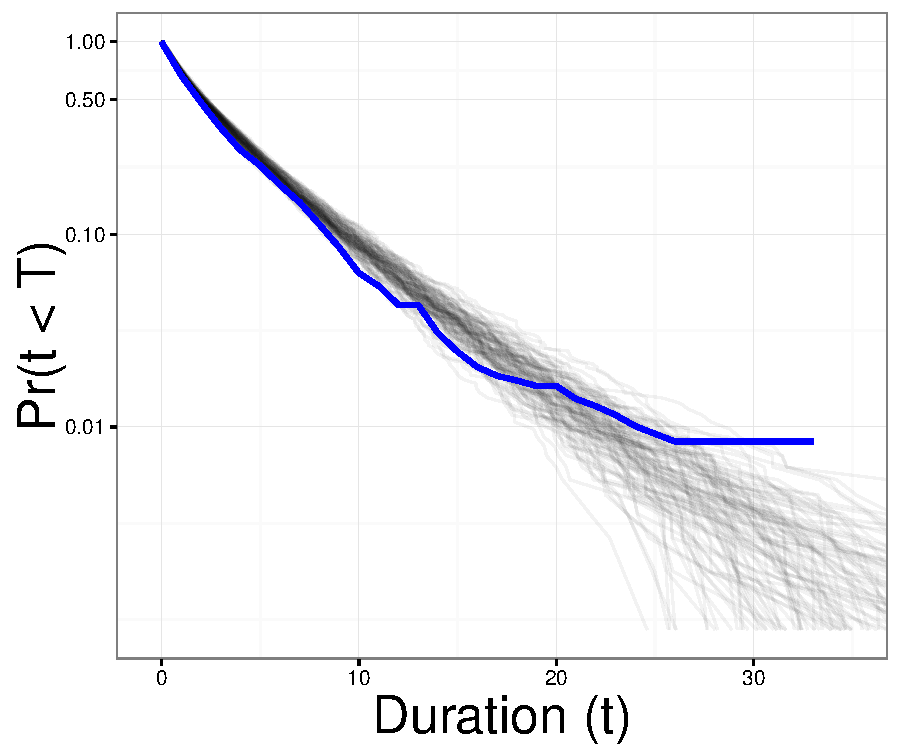
\includegraphics[height = 0.5\textheight,width=\textwidth,keepaspectratio=true]{figure/survival_curves}
  \caption{Comparison of the empirical estimate of \(S(t)\) (highlighted) versus estimates from 100 posterior predictive data sets (black). \(S(t)\) corresponds to the probability that the age of a genus \(t\) is less than the genus' ultimate duration \(T\). The vertical axis is log10 transformed.}
  \label{fig:surv}
\end{figure}


\begin{figure}[ht]
  \centering
  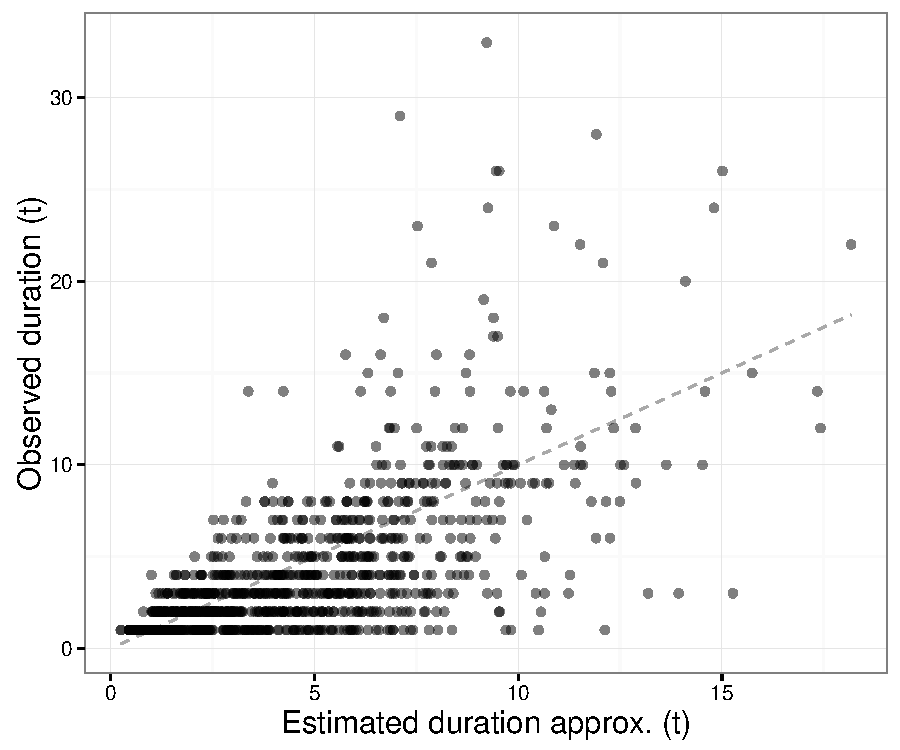
\includegraphics[height = 0.5\textheight,width=\textwidth,keepaspectratio=true]{figure/shotgun}
  \caption{Comparison of all observed genus durations in number of geological stages to the average posterior predictive estimates of \(\log(\sigma)\). The dashed, diagonal line corresponds to \(x = y\).}
  \label{fig:shot}
\end{figure}


\begin{figure}[ht]
  \centering
  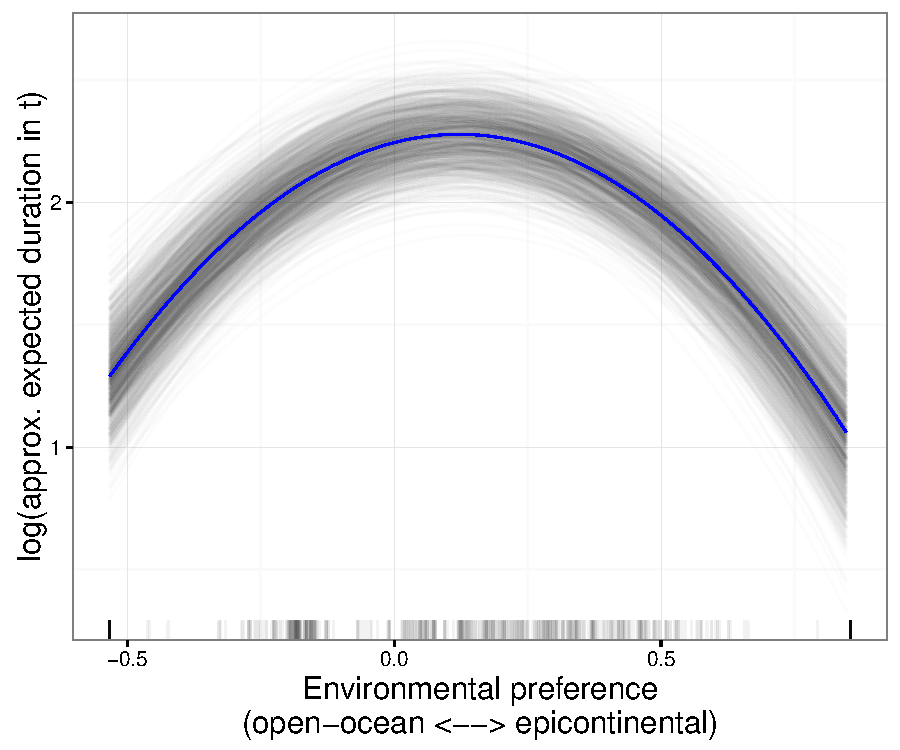
\includegraphics[height = 0.5\textheight,width=\textwidth,keepaspectratio=true]{figure/env_effect}
  \caption{The overall expected relationship between environmental affinity \(v_{i}\) and a \(\log(\sigma)\) when r = 0 and m = 0. The 1000 semi-transparent lines corresponds to a single draw from the posterior predictive distribution, while the highlighted line corresponds to the median of the posterior predictive distribution. The overall relationship is concave down with an optimum greater than 0, which means that taxa favoring epicontinental environments are expected to have longer durations than those favoring open-ocean environments. The tick marks along the bottom of the plot correspond to the (rescaled) observed values of environmental preference.}
  \label{fig:env_mean}
\end{figure}


\begin{figure}[ht]
  \centering
  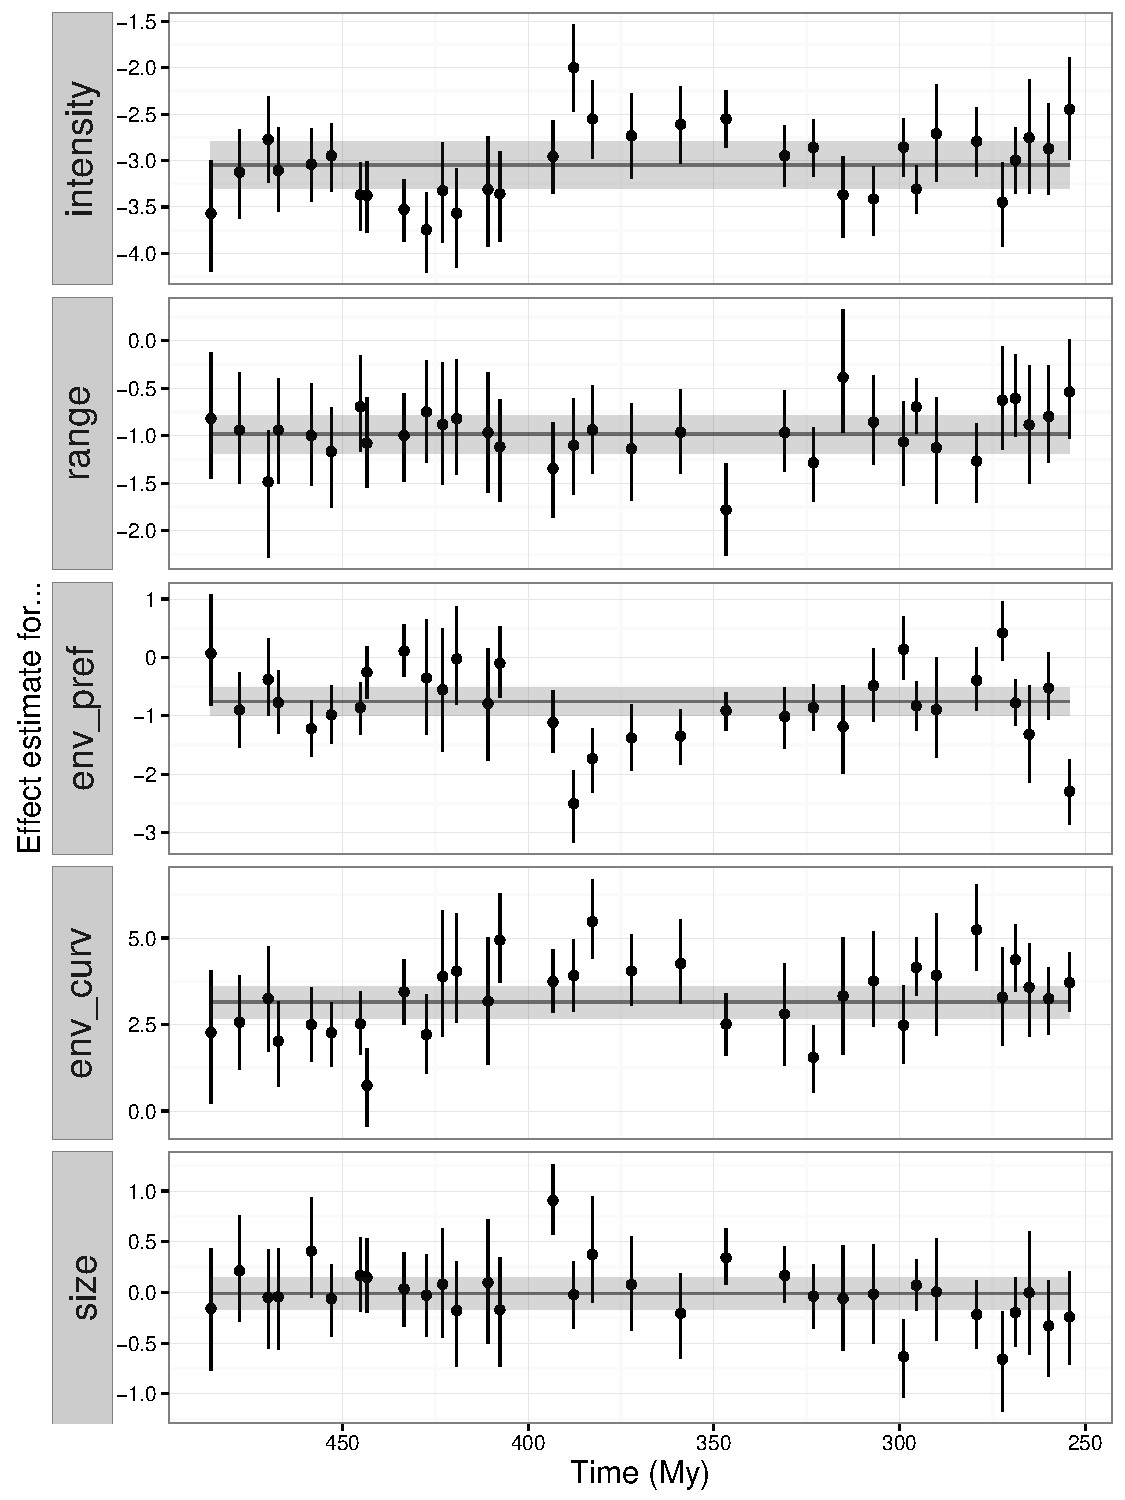
\includegraphics[width = \textwidth,height = 0.8\textheight,keepaspectratio=true]{figure/cohort_series}
  \caption{Comparison of cohort-specific estimates of \(\beta^{0}\), the effect of geographic range on extinction risk \(\beta^{r}\), the effect of environmental preference \(\beta^{v}\) and \(\beta^{v^{2}}\), and body size \(\beta^{m}\). Points correspond to the median of the cohort-specific estimate, along with 80\% credible intervals. Points are plotted at the midpoint of the cohorts stage of origination in millions of years before present (My). Black, horizontal lines are the overall estimates of covariate effects along with 80\% credible intervals (shaded).}
  \label{fig:cohort_series}
\end{figure}


\begin{figure}[ht]
  \centering
  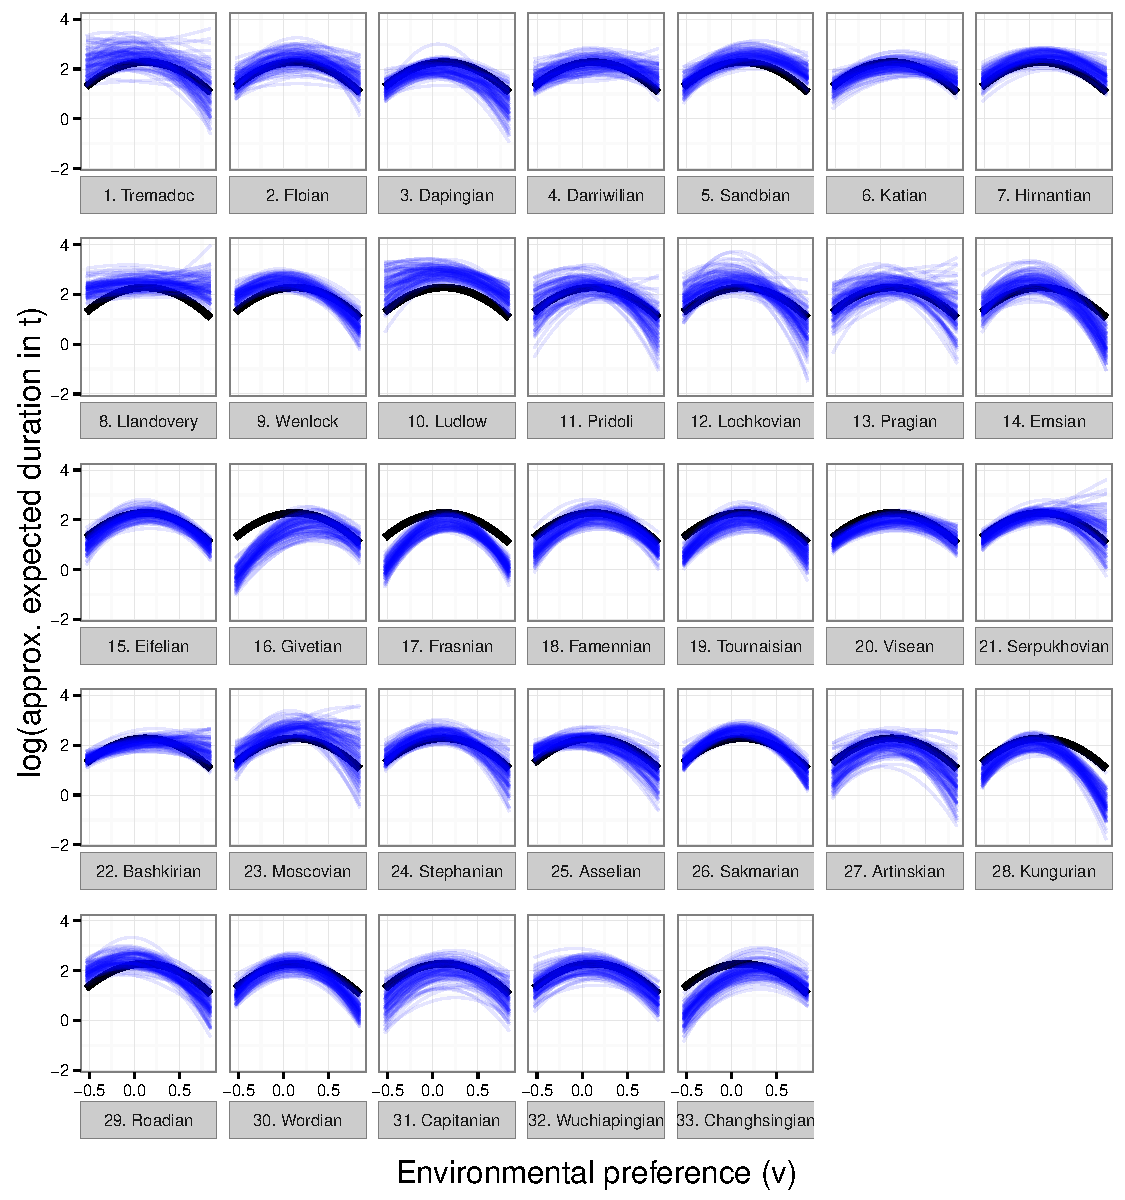
\includegraphics[width = \textwidth,height = 0.8\textheight,keepaspectratio=true]{figure/env_cohort}
  \caption{Comparison of origination cohort-specific (posterior predictive) estimates of the effect of environmental preference on \(\log(\sigma)\) to the mean overall estimate of the effect of environmental preference. Cohort-specific estimates are from 100 posterior predictive simulations across the range of (transformed and rescaled) observed values of environmental preference. The oldest cohort is in the top-right and younger cohorts proceed left to right, with the youngest cohort being the right-most facet of the last row. Panel names correspond to the name of the stage in which that cohort originated.}
  \label{fig:env_cohort}
\end{figure}


\begin{figure}[ht]
  \centering
  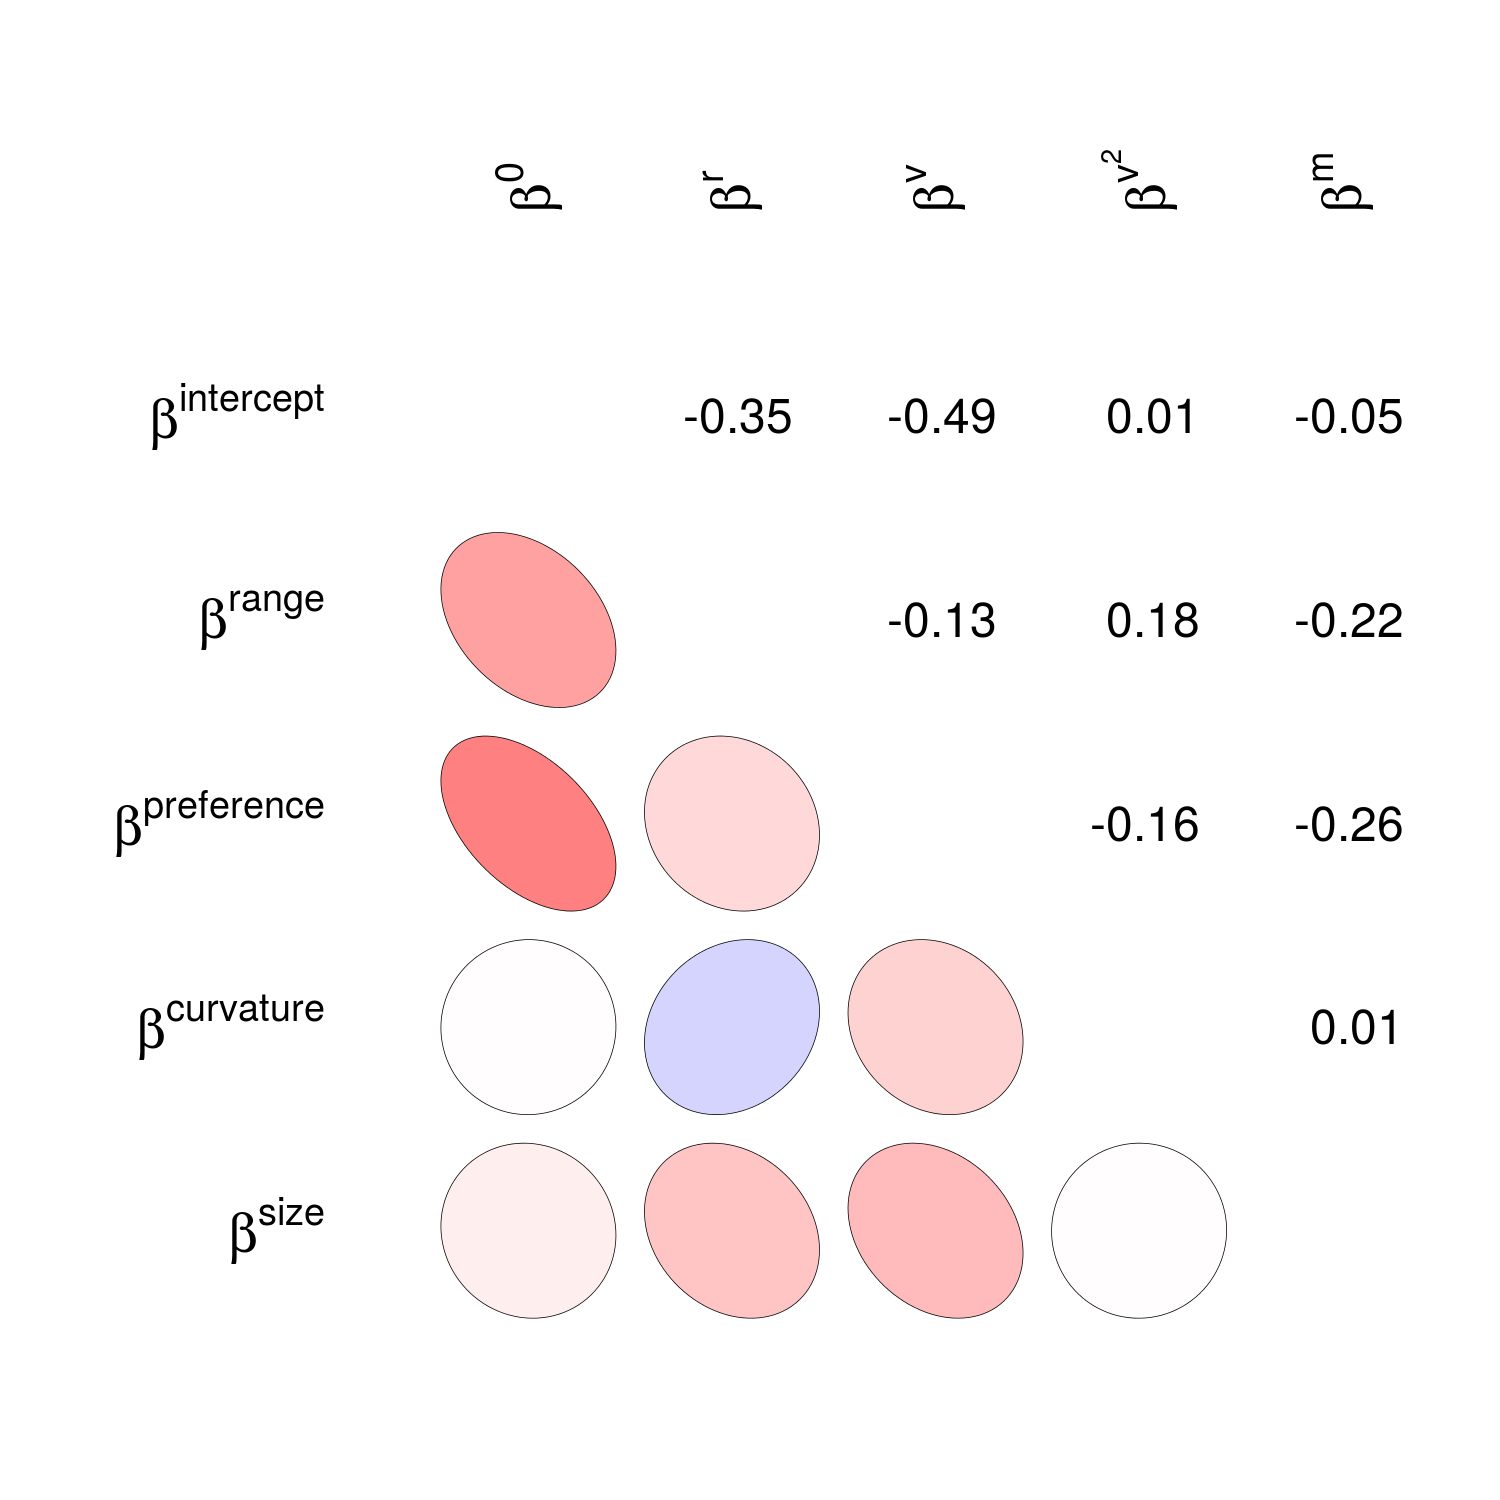
\includegraphics[height = 0.8\textheight,width=\textwidth,keepaspectratio=true]{figure/wei_cor_heatmap}
  \caption{Mixed graphical and numerical representation of the correlation matrix \(\Omega\) of variation in cohort-specific covariate estimates. These correlations are between the estimates of the cohort-level effects of covariates, along with intercept/baseline extinction risk. The median estimates of the correlations are presented numerically (upper-triangle) and as idealized ellipses representing that much correlation (lower-triangle). The darkness of the ellipse corresponds to the magnitude of the correlation.}
  \label{fig:cor_posterior}
\end{figure}

\begin{figure}[ht]
  \centering
  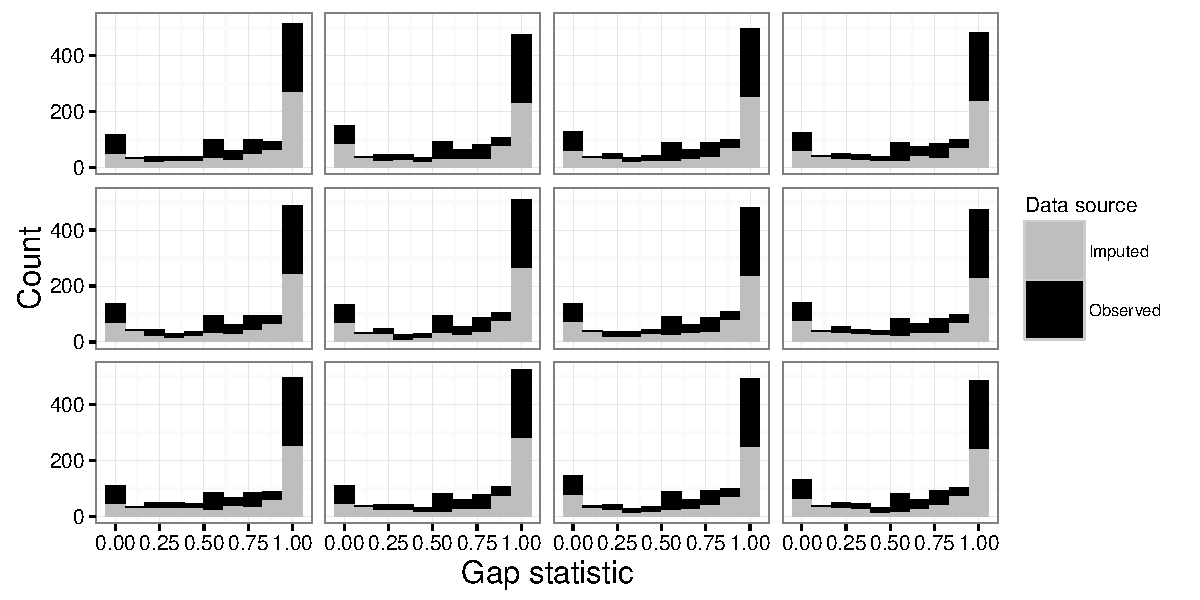
\includegraphics[height = 0.8\textheight,width=\textwidth,keepaspectratio=true]{figure/imputation_compare}
  \caption{Histograms of the distribution of gap statistic values from both the observed values and the imputed values from 12 unique posterior realizations. For each panel the observed values are identical but the imputed values are from a single set of their posterior estimates.}
  \label{fig:impute_results}
\end{figure}

\end{document}

